\chapter{Conformal Field Theory and Conformal Blocks}

The ubiquitous nature of conformal field theories in Theoretical and Mathematical physics has lead to their extensive study in the past years. Conformal field theories describe worldsheet dynamics in string theory, describe statistical systems at points of second order phase transitions and appear as renormalization group fixed points of quantum field theories.

A conformal field theory is a quantum field theory that is invariant under local conformal transformations. Conformal transformations are the transformations that preserve angles, but not necessarily lengths. The Lorentz transformations naturally preserve angles between spacetime vectors and thus form a subset of conformal transformations, therefore, the Lorentz group is a subgroup of the conformal group. The particle states in the theory then fit in irreducible representations of the conformal group. Since conformal invariance implies scale invariance the particle excitations in the theory have to be massless. This section gives a brief review of the general properties of conformal field theory.

  \section{Part I: Review of Conformal Field Theory}
  \subsection{The Conformal Group}
  We would like to find the set of all conformal transformations. A local conformal transformation is equivalently defined as a local coordinate transformation $x\xrightarrow{\Lambda(x)}x^\prime = \Lambda(x)x $ such that the metric components transforms as:
  \begin{align}
   g_{\mu\nu}(x) \xrightarrow{\Lambda(x)} g^\prime_{\mu\nu}(x^\prime) = \Omega^2(x) g_{\mu\nu}(x)  \label{ch2:metrictransform}
  \end{align}
  Lets see what this implies for the coordinate transformations. For now we work in $D-$dimensional euclidean space. Consider the infinitesimal coordinate transformation $x^\mu \to \tilde{x}^\mu=x^\mu + \epsilon^\mu(x)$ (Infinitesimal meaning ignoring terms of the order $\epsilon^2$ and $(\partial \epsilon)^2$). The metric components $g_{\mu\nu}$ transforms as:
  \begin{align}
   g_{\mu\nu}(x)\to \tilde{g}_{\mu\nu}(\tilde{x}) &= \frac{\partial x^\alpha}{\partial \tilde{x}^\mu}\frac{\partial x^\beta}{\partial \tilde{x}^\nu} \tensor[]{g}{_\alpha_\beta}(x) \\
   &= (\tensor[]{\delta}{^\alpha_\mu}-\tensor[]{\epsilon}{^\alpha_{,\mu}})(\tensor[]{\delta}{^\beta_\nu}-\tensor[]{\epsilon}{^\beta_{,\nu}})\tensor[]{g}{_\alpha_\beta}(x) \\
   &= \tensor[]{g}{_\mu_\nu}(x)-\tensor[]{\epsilon}{^\beta_{,\nu}}\tensor[]{g}{_\mu_\beta}(x)-\tensor[]{\epsilon}{^\alpha_{,\mu}}\tensor[]{g}{_\alpha_\nu}(x)
  \end{align}
  Plugging in $g_{\mu\nu}(x)=\delta_{\mu\nu}$ for euclidean space we get and using the metric transformation law $\tilde{g}_{\mu\nu}(\tilde{x}) = \Omega^2(x)\delta_{\mu\nu}$ for conformal transformations:
  \begin{align}
   \tilde{g}_{\mu\nu}(\tilde{x}) = \Omega^2(x)\delta_{\mu\nu} &= \delta_{\mu\nu}-\tensor[]{\epsilon}{_\mu_{,\nu}}-\tensor[]{\epsilon}{_\nu_{,\mu}} \\
   \implies \tensor[]{\epsilon}{_\mu_{,\nu}}+\tensor[]{\epsilon}{_\nu_{,\mu}} &= (\Omega^2(x)-1)\delta_{\mu\nu} \\
   2\tensor[]{\epsilon}{_\mu_{,\mu}} &= D (\Omega^2(x)-1) \\
   \tensor[]{\epsilon}{_\mu_{,\nu}}+\tensor[]{\epsilon}{_\nu_{,\mu}} &= \frac{2}{D}(\partial \cdot \epsilon) \delta_{\mu\nu} \label{2dconclusion}  
  \end{align}
  Acting on this with $\partial^\mu \partial^\alpha$ gives:
  \begin{align}
   \Box( \partial_\alpha \epsilon_\nu) = \partial_\alpha \partial_\nu \left( \frac{2}{D}-1\right) (\partial \cdot \epsilon) \label{eqconf1}
  \end{align}
  and acting with $\Box$ gives
  \begin{align}
   \delta_{\mu\nu} \Box (\partial \cdot \epsilon) = \frac{D}{2} \Box (\partial_\mu \epsilon_\nu + \partial_\nu \epsilon_\mu) \label{eqconf2}
  \end{align}
Now we get from (\ref{eqconf1}) and (\ref{eqconf2}):
\begin{align}
 \left(\Box \delta_{\mu\nu} + (D-2)\partial_\mu \partial_\nu \right)(\partial \cdot \epsilon) = 0 \label{eqconf3}
\end{align}
Lets consider the cases $D=2$ and $D > 2$ separately
\subsubsection{\underline{$D > 2$}}
We see from (\ref{eqconf3}) that all 2nd derivatives of $\partial \cdot \epsilon$ must vanish, that is its most general form is:
\begin{align}
 \partial \cdot \epsilon &= a + b_\mu  x^\mu \\
 \implies \epsilon^\mu &= c^\mu + \tensor[]{d}{^\mu_\alpha} x^\alpha + \tensor[]{e}{^\mu_{\alpha\beta}} x^\alpha x^\beta \qquad , \tensor[]{e}{^\mu_{\alpha\beta}}=\tensor[]{e}{^\mu_{\beta\alpha}}
\end{align}
These infinitesimal transformations can be classified in 4 qualitatively different \emph{classes} of solutions, namely: translations, rotations, dilatations and special conformal transformations, with their associated generators: 

\begin{table}[h!]
  \centering
  \caption{Infinitesimal conformal transformations and generators.}
  \label{ch2:table1}
  \begin{tabular}{ccc}
    \toprule
    Transformation & Action & Generator\\
    \midrule
    $\epsilon^\mu = c^\mu $ & Translation & $P_\mu = -i \partial_\mu$\\
    $\epsilon^\mu =  \tensor[]{\omega}{^\mu_\alpha} x^\alpha$ & Rigid rotation & $ M_{\mu\nu}=i(x_\mu\partial_\nu - x_\nu \partial_\mu)$ \\
    $\epsilon^\mu = \lambda x^\mu$ & dilation & $D=-i x^\mu \partial_\mu$\\
    $\epsilon^\mu = 2(b\cdot x) x^\mu - b^\mu x^2$ & SCT & $K_\mu=-i(2x_\mu x^\nu \partial_\nu-x^2 \partial_\mu)$
%    \bottomrule
  \end{tabular}
\end{table}

The integrated transformations read:

\begin{table}[h!]
  \centering
  \caption{Finite conformal transformations and scale factors.}
  \label{ch2:table2}
  \begin{tabular}{ccc}
    \toprule
    Transformation & Action & Scale factor\\
    \midrule
    $\tilde{x}^\mu = x^\mu +a^\mu $ & Translation & $1$\\
    $\tilde{x}^\mu = \tensor[]{M}{^\mu_\nu}x^\nu$ & Rigid rotation & $1$\\
    $\tilde{x}^\mu = \lambda x^\mu$ & dilation & $ \lambda^2$\\
    $\tilde{x}^\mu = \frac{x^\mu -b^\mu x^2}{1-2b\cdot x +b^2 x^2}$ & SCT & $(1-2b\cdot x +b^2 x^2)^2$
   % \bottomrule
  \end{tabular}
\end{table}


  These generators obey the following commutation relations:
  
  \begin{align*}
  \centering %Note for centering??
  [D,K_{\mu}] &= -iK_{\mu} \\
  [D,P_{\mu}] &= iP_{\mu} \\
  [K_{\mu},P_\nu] &= 2i\eta_{\mu\nu} D - 2iM_{\mu\nu} \\
  [K_\mu,M_{\rho\sigma}] &= i(\eta_{\mu\rho}K_\sigma - \eta_{\mu\sigma}K_{\rho}) \\
  [P_\mu, M_{\rho\sigma}] &= i(\eta_{\mu\rho}P_\sigma - \eta_{\mu\sigma}P_{\rho}) \\
   [M_{\mu\nu},M_{\rho\sigma}] &= i(\eta_{\nu\rho}M_{\mu\sigma}+\eta_{\mu\sigma}M_{\nu\rho}-\eta_{\mu\rho}M_{\nu\sigma}-\eta_{\nu\sigma}M_{\mu\rho})
  \end{align*}
  
  \subsubsection{\underline{$D = 2$}}
  In $D=2$ the story is slightly different. This is because for $D=2$, (\ref{eqconf3}) reads:
  \begin{align}
   \Box (\partial \cdot \epsilon ) = 0
  \end{align}
  In this case it is easier to draw conclusions from the first order differential equation (\ref{2dconclusion}):
  
  \begin{align}
   \tensor[]{\epsilon}{_\mu_{,\nu}}+\tensor[]{\epsilon}{_\nu_{,\mu}} &= \frac{2}{D}(\partial \cdot \epsilon) \delta_{\mu\nu}
  \end{align}
  For $\mu =\nu =x$ and $\mu=x,\nu=y$ respectively we get the equations:
  \begin{align}
   \frac{\partial \epsilon_x}{\partial x} &= \frac{\partial \epsilon_y}{\partial y} \label{ch2:cr1}\\
   \frac{\partial \epsilon_x}{\partial y} &= -\frac{\partial \epsilon_y}{\partial x} \label{ch2:cr2}
   \end{align}
  Switching to complex coordinates $(x,y) \to (z,\bar{z})$ and writing $\epsilon(z)=\epsilon_x+i\epsilon_y$ and $\bar \epsilon(\bar{z})=\epsilon_x-i\epsilon_y$, equations (\ref{ch2:cr1}) - (\ref{ch2:cr2}) are the Cauchy-Riemann equations and imply holomorphicity and anti-holomorphicity for $\epsilon(z)$ and  $\bar \epsilon(\bar{z})$ respectively for all $z,\bar z$. 
  
  Since this implies that $f=z+\epsilon$ and $\bar f = \bar z +\bar \epsilon$ are holomorphic and antiholomorphic for all $z,\bar z$ one concludes that the set of transformations $z \to f(z)$ and  $\bar z \to \bar f(\bar z)$ with $f$ and $\bar f$ holomorphic and anti-holomorphic satisfies the conformality condition (\ref{ch2:metrictransform}) in 2 dimensions.
  
  The $D=2$ conformal algebra is infinite dimensional, in contrast to the $D>2$ case. The generators are given by
  
  \begin{align}
   l_m = -z^{m+1}\partial_z, \quad \bar{l}_m = -\bar{z}^{m+1} \partial_{\bar{z}} \qquad (m \in \mathbb{Z})
  \end{align}
  Satisfying 
  \begin{align}
   [l_m,l_n] =(m-n) l_{m+n}, \quad [\bar{l}_m,\bar{l}_n] =(m-n) \bar{l}_{m+n} \label{ch2:witt}
  \end{align}
  The algebra (\ref{ch2:witt}) is known as the Witt Algebra. Note that so far we have only considered classical theories with conformal transformations. Upon quantizing the theory(in the next section), we will see that the algebra is usually altered. In particular for $D=2$ CFTs the symmetry algebra changes from the Witt algebra to its central extension, the Virasoro algebra:
  \begin{align}
   [L_m,L_n] &= (m-n)L_{m+n} + \frac{c}{12}n(n^2-1)\delta_{m+n,0} \\
   [\bar{L}_m,\bar{L}_n] &= (m-n)\bar{L}_{m+n} + \frac{\bar c}{12}n(n^2-1)\delta_{m+n,0} 
  \end{align}
  

  \subsection{Radial Quantization}
  
  \subsubsection{Brief Detour to Hilbert Space and Path Integrals in QFT}
  
  Consider a QFT defined by the Hamiltonian $H[\phi,\pi]$, where $\phi$ and $\pi$ are the field and conjugate momentum respectively. As in canonical quantization of a QFT, one may foliate spacetime into spacelike slices of constant time(see figure \ref{ch2:foliatefig}) with each slice endowed with its own Hilbert space. This Hilbert space has basis states labeled by field configurations at a fixed time $t_0$ i.e. states of the form $\left\lbrace \, \ket{\{\phi(\bold{x},t_0)\}} \,\right\rbrace$. The notation $\ket{\{\phi(\bold{x},t_0)\}}$ is meant to denote the fact that the entire spatial configuration $\{\phi(\bold{x},t_0)\}$ for \textbf{all} $\bold{x}$ and constant time $t=t_0$ corresponds to \textbf{one} state in the Hilbert space. These states are eigenstates of the the field operator, and acting on them with the \textbf{local} operator $\hat{\phi}(\bold{x},t_0)$ gives the local value of the classical field $\phi(\bold{x},t_0)$ at the point $(\bold{x},t_0)$:
  
  \begin{align}
   \hat{\phi}(\bold{x},t_0) \ket{\{\phi(\bold{x},t_0)\}} = \phi(\bold{x},t_0) \ket{\{\phi(\bold{x},t_0)\}} 
  \end{align}

  
  
  
  The probability amplitude for the field to evolve from an initial field configuration $\phi(\bold{x},0) = \phi(\bold x)$ at $t=0$ to a final field configuration $\phi(\bold{x},t) = \phi^\prime(\bold x)$ at $t=t$ is given by the path integral:
  \begin{align}
   S_{f \leftarrow i} = \tensor[_t]{\braket{\phi^\prime | e^{-it \hat{H}} | \phi}}{_0} = \int_{\phi(\bold{x},0) = \phi(\bold x)}^{\phi(\bold{x},t) = \phi^\prime(\bold x)} \mathcal{D} \phi e^{-\frac{1}{\hbar}S[\phi] }
  \end{align}
  
  %\int_0^t \mathrm{d}t^\prime \int \mathrm{d}^3 \bold{x} \left( \pi \dot{\phi} - H[\pi,\phi] \right)
  Where the integration over $\pi$ can be performed after plugging in a Hamiltonian of the form
  
  Now, one can write a state on some slice $t=t_1$ 
  
  \begin{align}
   H=\frac{1}{2}\pi^2 + \frac{1}{2}(\nabla \phi)^2 + V(\phi)
 \end{align}
  to get
  \begin{align} \label{ch2:transition_amplitude}
   \braket{\phi^\prime | e^{-it \hat{H}} | \phi} = \int_{\phi(\bold{x},0) = \phi(\bold x)}^{\phi(\bold{x},t) = \phi^\prime(\bold x)} \mathcal{D} \phi e^{\frac{i}{\hbar} \int_0^t \mathrm{d}t^\prime \int \mathrm{d}^3 \bold{x} \mathcal{L}[\phi,\partial \phi]}
  \end{align}
  
  
  

  \begin{figure}
\centering
  
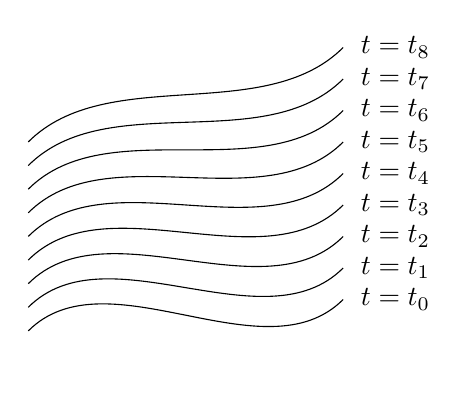
\begin{tikzpicture}
\foreach \s in {0,...,8}
{
\coordinate (A) at (0,0.3*\s);
\draw (A)  ..controls ++(1,1) and ++(-1,-1) .. ++(4,{0.4+0.1*\s}) node[right = 1mm] {$t=t_\s$}; %.. controls (1,4) and (3,0)
}
\end{tikzpicture}

  \caption{A foliation of spacetime in space-like slices along the time direction, with $t_i < t_j \forall i<j$.}
  \label{ch2:foliatefig}
\end{figure}  
  
  
  The organizing principle in usual QFT is labeling the representations with the eigenvalues of the casimir operators of the Poincar\'{e} algebra, $C_1=P_\mu P^\mu$ and $C_2=W_\mu W^\mu$, where $W_\mu$ is the Pauli-Lubanski operator. In a CFT however the operator $C_1$ is no longer a casimir, since it doesn't commute with, say, the generators of dilatations, $D$. If a representation contains a state with a fixed energy, due to scale invariance one can rescale the mass and energy by some constant factor and so the representation contains states of all energies. Therefore classification of states with respect to mass/energy is not feasible and moreover, in general for a CFT the hamiltonian, $P^0$ in general has a continuous spectrum. Instead, the dilatation operator $D$ plays the role of the Hamiltonian, and states in the Hilbert space live on surfaces of constant radius $r=r_0$ instead of constant time $t=t_0$. In direct analogy with the preceding discussion and eq. (\ref{ch2:transition_amplitude}) for general QFTs, the state $\ket{\{h_0(r=r_0)\}}$ living on the sphere $r=r_0$ evolves into the state $\ket{\{h_1(r=r_1)\}}$ given by:
  \begin{align} 
   \ket{\{h_1(r=r_1)\}} &= e^{-\beta D} \ket{\{h_0(r=r_0)\}} \label{ch2:radial_transition_amplitude_1} \\
			&= \mathbb{1} \, e^{-\beta D} \ket{\{h_0(r=r_0)\}} \\
			&= \int [\mathcal{D}h(r_1)] \ket{\{h(r_1)\}} \braket{\{ h(r_1)\}| e^{-\beta D} |\{h_0(r_0)\}} \\
			&= \int [\mathcal{D}h(r_1)] \ket{\{h(r_1)\}} \int_{\tilde{h}(r=r_0)=h_0(r_0)}^{\tilde{h}(r=r_1)=h(r_1)}[\mathcal{D}\tilde{h}] e^{-S[\tilde{h}]}  \\
			&= \left(\int_{h(r=r_0)=h_0(r_0)} [\mathcal{D}h(r_0 \leqslant r \leqslant r_1)] e^{-S[h]} \right) \ket{\{h(r_1)\}} \label{ch2:radial_transition_amplitude_2}
  \end{align}
  In particular one may ``create'' the vacuum state $\ket{0}$ using the path integral. Recall that in the limit that $\beta \to \infty$, the evolution operator (or transfer matrix, in statistical physics) $e^{-\beta \hat{D}}$ projects onto the ground state:
  \begin{align}
  e^{-\beta \hat{D}} \xrightarrow{\beta \to \infty} e^{-\beta E_0} \ket{0}\bra{0}
  \end{align}
  
  Since $r \to 0$ corresponds to taking the euclidean time $\tau \to -\infty \implies \beta \to \infty$, we have with eq.(\ref{ch2:radial_transition_amplitude_1} - \ref{ch2:radial_transition_amplitude_2}):
  \begin{align} 
   \ket{0} =\lim_{r_0\to \infty} \int [\mathcal{D}h_0(r_0)]\int [\mathcal{D}h(r_1)] \ket{\{h(r_1)\}} \int_{\tilde{h}(r=r_0)=h_0(r_0)}^{\tilde{h}(r=r_1)=h(r_1)}[\mathcal{D}\tilde{h}] e^{-S[\tilde{h}]} \label{ch2:radial_transition_amplitude_3}
  \end{align}
  
  This can be represented in the following form with the understanding that the boundary value configurations given by $h(r=r_1)$ are integrated over:
  
  \begin{align} \label{ch2:vac}
   \ket{0} = \int [\mathcal{D}h(r \leqslant r_1)] e^{-S[h]} \ket{\{h(r_1)\}}
  \end{align}

  
  With this expression in hand, we are set to discuss the \textbf{state-operator correspondence}.
  
  \subsubsection{State-Operator Correspondence}
  The State-Operator correspondence in CFT is a one-to-one correspondence between Hilbert space states living on the surface of some radius $r_0$ and operators inserted at the origin, or more generally anywhere in the region $r \leqslant r_0$. 
  
  
  
  \begin{enumerate}
   \item \textbf{Operator $\rightarrow$ State} Inserting an operator $\hat{\mathcal{O}}_{\Delta}(0)$ at the origin creates an eigenstate of the dilatation operator $\hat D$ on the sphere of radius $r_0$. In eq.(\ref{ch2:vac}) this corresponds simply to an insertion of the operator in the path integral:
   \begin{align}
   \hat{\mathcal{O}}_{\Delta}(0) \ket{0} = \left(\int [\mathcal{D}h(r \leqslant r_1)] \mathcal{O}_\Delta (0) e^{-S[h]} \right)\ket{\{h(r_1)\}}
   \end{align}
   \begin{align}
    \hat D \hat{\mathcal{O}}_{\Delta}(0) \ket{0} &= [\hat D , \hat{\mathcal{O}}_{\Delta}(0)] \ket{0} +  \cancelto{0}{\hat{\mathcal{O}}_{\Delta}(0) \hat D \ket{0}} \\
    &=\lim_{x\to 0} (\Delta -ix^\mu \partial_\mu) \hat{\mathcal{O}}_{\Delta}(x) \ket{0} \\
    &=\Delta \hat{\mathcal{O}}_{\Delta}(x) \ket{0}
   \end{align}
  
  Moreover, inserting an operator $\hat{\mathcal{O}}_{\Delta}(x)$ at a point $x$ inside the sphere of radius $r_0$, i.e. $0<|x|<r_0$ does not produce an eigenstate of the dilatation operator but since it is still a state in the Hilbert space it may be expanded in $\hat D$ eigenstates. This can be seen using the fact that $\hat P^\mu$ generates translations along $x^\mu$ and therefore $\hat{\mathcal{O}}_{\Delta}(x)= e^{i\hat{P}\cdot x}\hat{\mathcal{O}}_{\Delta}(0) e^{-i\hat{P}\cdot x}$ which gives:
  
  \begin{align}
   \hat{\mathcal{O}}_{\Delta}(x) \ket{0} &= e^{i\hat{P}\cdot x}\hat{\mathcal{O}}_{\Delta}(0) e^{-i\hat{P}\cdot x} \ket{0} \\
   &=e^{i\hat{P}\cdot x}\hat{\mathcal{O}}_{\Delta}(0) \ket{0} \\
   &=e^{i\hat{P}\cdot x} \ket{\Delta} \\
   &=\sum_{n=0}^\infty \frac{(i\hat{P}\cdot x)^n}{n!} \ket{\Delta} \\
   &= c_0(x) \ket{\Delta} + c_1(x) \ket{\Delta+1} +c_2(x) \ket{\Delta+2} \dots
  \end{align}
  Where in the second line we have used the uniqueness and conformal invariance of the vacuum $\ket{0}$ implying $\hat{P}^\mu \ket{0} = 0$. Therefore the only term surviving in  $e^{-i\hat{P}\cdot x} \ket{0}$ is the first term $\mathbb{1}\ket{0}$ with the identity operator. In the last line we have used the fact that $\hat{P}^\mu$ are raising operators for $\hat D$ eigenstates. This means $\hat P \ket{\Delta} \sim \ket{\Delta+1}, \hat{P}^2 \ket{\Delta} \sim \ket{\Delta+2}$ and so on.
  
  Another way to reach the same conclusion is using the path integral expression (\ref{ch2:vac}):
  \begin{align}
   \ket{\Psi}=\hat{\mathcal{O}}_{\Delta}(x) \ket{0} = \underbrace{\left(\int [\mathcal{D}h(r \leqslant r_1)] \mathcal{O}_\Delta (x) e^{-S[h]} \right)}_{\text{I}}\ket{\{h(r_1)\}}
   \end{align}
   
   The path integral (I) we can taylor expand $\mathcal{O}_\Delta (x)$ around $x=0$ to give:
  \begin{multline}
   \ket{\Psi} = \bigg( \int [\mathcal{D}h(r \leqslant r_1)] \bigg\lbrace \mathcal{O}_\Delta (0) + \frac{x}{1!}\partial \mathcal{O}_\Delta (0)  \\ 
   + \frac{x^2}{2!}\partial^2 \mathcal{O}_\Delta (0)+\dots \bigg\rbrace e^{-S[h]} \bigg)\ket{\{h(r_1)\}}
   \end{multline} 
   \begin{align}
    \implies \ket{\Psi} &= \sum_{n=0}^{\infty} \frac{(ix\hat P)^n}{n!}\bigg( \int [\mathcal{D}h(r \leqslant r_1)]  \mathcal{O}_\Delta (0) e^{-S[h]} \bigg)\ket{\{h(r_1)\}} \\
    \ket{\Psi} &= \sum_{n=0}^{\infty} \frac{(ix\hat P)^n}{n!} \hat{\mathcal{O}}_\Delta(0)\ket{0} \\
    \ket{\Psi} &= \sum_{n=0}^{\infty} \frac{(ix\hat P)^n}{n!} \ket{\Delta}
   \end{align}
  \item \textbf{State $\rightarrow$ Operator} Given a state $\ket{\psi}$ on a sphere of radius $r_0$ (in radial quantization), one can cut out a small sphere $S_\epsilon$ of radius $\epsilon$ at the origin with the boundary conditions on $S_\epsilon$ defined by $\ket{\psi}$ in the following sense: using the eqn. (\ref{ch2:radial_transition_amplitude_2}) one writes the state $\ket{\psi}$ as:
  
  \begin{align}
   \ket{\psi} = \left( \int_{h(\epsilon)=h_0(\epsilon)} [\mathcal{D}h(\epsilon \leqslant r \leqslant r_0)]   e^{-S[\tilde{h}]} \right) \ket{\{h(r_1)\}}
  \end{align}
  Where the initial state $\ket{\{h_0(\epsilon)\}}$ is determined uniquely given $\ket{\psi}$. Due to conformal invariance the absolute size of $r_0$ does not matter. Additionally in contrast to a QFT without conformal invariance one can take the limit $\epsilon \to 0$ and then the state $\ket{\{h_0(\epsilon)\}}$ defines uniquely an operator $\hat{\mathcal{O}}_{\ket{\psi}}(0)$ as:
  
  \begin{align}
   \lim_{\epsilon \to 0} \ket{\{h_0(\epsilon)\}} = \lim_{\epsilon \to 0}\hat{\mathcal{O}}_{\ket{\psi}}(\epsilon) \ket{0}
  \end{align}
  In particular, a given $\hat{D}$ eigenstate $\ket{\Delta}$ on some sphere $S_{r_0}$ corresponds uniquely to the operator insertion $\op{O}_\Delta(0)$ at the origin independent of the radius $r_0$.
   \end{enumerate}
  
  
%   
%   
%   
%   
%   States are classified according to their scaling dimension $\Delta$ under the dilatation operator $D$. Since $P^\mu$ and $K^\mu$ act as raising and lowering operators respectively, for each $\Delta$ we have a lowest ``energy'' state $\ket{\Delta}$ called the \emph{\textbf{primary}} which is annhilated by the lowering operator:
%   \begin{align}
%    K^\mu \ket{\Delta} = 0
%   \end{align}
%   Each such primary, along with all states obtained by succesive applications of the raising operator $P^\mu$, called the \emph{\textbf{descendant}} states furnishes a representation of the conformal algebra. 
%   
%   [check Tong -string theory+cardy les houches]
%   As we discussed before, one of the features of a Conformal field theory is that there is no inherent mass scale in the theory. Therfore, the hamiltonian ends up having a continuum of eigenstates and the usual quantisation on the line is not so useful since one cannot define asymptotic states in the usual way. We will see that just as in usual QFTs one utilises the time-translation invariance, to foliate spacetime into equal time slices and quantise the theory on these qual time slices, in a CFT it is more natural to use the scale invariance of the theory, and quantise it on circles of equal radii $r_0$. The nthe role played by the Hamiltonian (generator of time translations) is replaced by $D$ the generator of dilatations (scale transformations). Then $D$ has a discrete spectrum. So far we have discussed the canonical picture. 
%   
%   
%   
% 
%   
%   In the path integral formulation, the Hilbert space of such a CFT would correspond to the space of field configurations $\Ket{h(r_0,\theta)}$ on a circle of radius $r_0$ \cite{Cardy:2008jc}. [CLARIFY]. The vacuum state is given by
%   
%   
%   Let us discuss the Hilbert Space structure of QFTs. In canonical quantisation of a QFT, the usual procedure is to choose a foliation of space-time into spacelike slices of constant time. Each leaf of this foliation carries its own copy of Hilbert space.[insert diagram]. Since the Hilbert spaces on different slices are related by a symmetry transformation, namely that of time translation, generated by $P^0$, the Hilbert spaces are infact isomorphic and can be identified as the same Hilbert space. The Hamiltonian ($P^0$) and $P^i$ form a complete set of commuting operators (CSCO) in the Poincar\'{e} algebra, therefore we can classify states according to their eigenvalues i.e. the energy and momenta:
%   
%   \begin{align}
%    P^\mu \Ket{k^\mu} = k^\mu \Ket{k^\mu}
%   \end{align}
%   
%   
%   
%   
%   
%   Then there exists a vacuum state $\left| \text{VAC} \right\rangle$ which is annhilated by the lowering operator, and \emph{fields} or \emph{field operators} map one state in the Hilbert space into another state. For two states, $\left| \psi_1 \right\rangle$ and $\left| \psi_2 \right\rangle$ on the same slice, the probability of one state evolving into another is given by the overlap of these $\left\langle \psi_2 | \psi_1 \right\rangle$, and this also measures the correlator of the two operators which generate these states. So if $\left| \psi_1 \right\rangle = \mathcal{O}_1 \left| \text{VAC} \right\rangle$ and $\left| \psi_2 \right\rangle = \mathcal{O}_2 \left| \text{VAC} \right\rangle$, then we have:
%   \begin{align*}
%    \left\langle \psi_2 | \psi_1 \right\rangle = \left\langle \mathcal{O}_2 \mathcal{O}_1 \right\rangle
%   \end{align*}
% 
%   
%   One may insert field operators on a particular time slice, and this may correspond to generating or measuring a particle. For example, one may insert a creation operator $a^{\dag}_p$ on the vacuum of the $t=-T$ slice to get the $\left| \text{in} \right\rangle$ state: 
%   \begin{align*}
%    \left| \text{in} \right\rangle= \left|\vec{p},-T \right\rangle = a^{\dag}_{\vec{p}} \left| \text{VAC}, -T \right\rangle
%   \end{align*}
% and similarly the out state on the  $t=+T$ 
% \begin{align*}
%  \left\langle \text{out} \right| = \left\langle \vec{q},T \right| = \left\langle \text{VAC}, T \right| a_{\vec{q}}
% \end{align*}
%   The time evolution operator $U(t_2,t_1)$ can propagate states from time slice $t_1$ to another time slice $t_2$ and thus we can calculate the probability amplitude of  project one state $\psi_1$ on another state $\psi_2$ and get the probability amplitude for this 
%   
%   One typically wants to study 2 dimensional CFTs on the cylinder since this is the natural home of a CFT for example in String Theory and moreover it removes IR divergences. This essentially amounts to compactifying the space direction using periodic boundary conditions (insert diagram). Now this 
%   
   
  \subsection{Operator Product Expansion}
  
  Let's go ahead and see a general derivation of the operator product expansion in CFTs from radial quantization. The crucial difference of the CFT OPE from general QFT OPE is the following: for a general QFT the OPE is an asymptotic expansion of the product of two operators $\phi_1(x_1), \phi_2(x_2)$ inside the correlator, in the limit when the two operators get arbitrarily close, $x_1 \to x_2$. However, in a CFT, the OPE is convergent and is an exact statement. Inside a correlator, the radius of convergence of the OPE is given by the next nearest operator insertion.
  
  \begin{figure}
\centering
\begin{tikzpicture}
\draw[dashed] (0,0) circle (3cm);
\coordinate (A) at (45:3);
\draw[fill] (0,0) node[below]{$\mathcal{O}_1(x_1)$} circle (0.05cm);
\draw[fill] (1.5,0.5) node[below]{$\mathcal{O}_2(x_2)$} circle (0.05cm);
\draw[fill] (A) node[right]{$\mathcal{O}_3(x_3)$} circle (0.05cm);
\draw[fill] (4,-1) node[below]{$\mathcal{O}_4(x_4)$} circle (0.05cm);
\end{tikzpicture}
\caption{The radius of convergence of the $\mathcal{O}_1\mathcal{O}_2$ OPE is determined by the next nearest operator insertion. In this case it is given by $r=|x_1-x_3|$.}
\end{figure}
  
  Using the path integral expressions of the State-Operator correspondence we can write for the state $\ket{\Psi}$(see fig. \ref{ch2:pic:OPEderive}):
  
  \begin{align}
   \ket{\Psi} = \hat{\mathcal{O}}_2(x) \hat{\mathcal{O}}_1(0) \ket{0} =\int [\mathcal{D}h(r\leqslant r_0)] \mathcal{O}_2(x) \mathcal{O}_1(0) e^{-S[h]} \ket{\{h(r_1)\}}
  \end{align}

  \begin{figure}
\label{ch2:pic:OPEderive}
\centering
\begin{tikzpicture}
\draw[dashed] (0,0) circle (3cm);
\coordinate (A) at (45:3);
\draw[fill] (0,0) node[below]{$\mathcal{O}_1(0)$} circle (0.05cm);
\draw[fill] (-1.7,0.8) node[below]{$\mathcal{O}_2(x)$} circle (0.05cm);
%\draw[fill] (A) node[right]{$\mathcal{O}_3(x_3)$} circle (0.05cm);
%\draw[fill] (4,-1) node[below]{$\mathcal{O}_4(x_4)$} circle (0.05cm);
\draw[fill] (A) node[right] {$\ket{\Psi}$};
\end{tikzpicture}
\caption{Derivation of the OPE using the State-Operator correspondence.}
\end{figure}
  
  This state $\ket{\Psi}$ being an element of the Hilbert space (and a function of the coordinate $x$) may be expanded in eigenvectors (primaries and descendants) of the operator $\hat D$, $D_n$
  
  \begin{align}
   \ket{\Psi} = \sum_{n} c_n(x) \ket{D_n}
  \end{align}

  Using the state-operator correspondence now we can associate each $\ket{D_n}$ either a \textbf{primary operator}  $\hat{\mathcal{O}}$ or some descendant $\partial^n \hat{\mathcal{O}}$:
  
  \begin{align} 
   \hat{\mathcal{O}}_2(x) \hat{\mathcal{O}}_1(0) \ket{0} &= \left(\sum_{{\mathcal{O}}} \sum_{n} c^{\mathcal{O}}_n(x,\partial^n) \hat{\mathcal{O}}(0) \right) \ket{0} \label{ch2:OPE_proof_1} \\
   &=\left(\sum_{{\mathcal{O}}}  \frac{\lambda_{21\mathcal{O}}}{|x|^k} [1+\frac{c_1}{2} x^\mu \partial_\mu +\frac{c_2}{8} x^\mu x^\nu \partial_\mu \partial_\nu + \dots]\op{O}_{\Delta}(0) \right) \ket{0} \label{ch2:OPE_proof_2}
  \end{align}
  Where the summation is over primaries $\op{O}$ and $[\dots]$ represent further descendants of the respective primaries which come with their own additional coefficients.

  Conformal symmetry makes the OPE even more powerful in that by requiring that both the LHS and RHS of eqn. (\ref{ch2:OPE_proof_1}) transform in the same way one can constrain the coefficients of particular operators in the OPE. In particular, by operating on both sides of \ref{ch2:OPE_proof_2} with $\hat D$ and matching the coefficients, one can fix the exponent $k$ for a scalar operator $\op{O}$ of dimension $\Delta$ in the OPE \ref{ch2:OPE_proof_2} to be $k=\Delta_1+\Delta_2-\Delta$, and by operating with $K^\mu$ recursively one can fix the constants $c_i$ exactly.
  \begin{multline}\label{ch2:OPE_final}
  \braket{\op{O}_1(x)\op{O}_2(0)}=\left(\sum_{{\mathcal{O}}}  \frac{\lambda_{21\mathcal{O}}}{|x|^{\Delta_1+\Delta_2 - \Delta}} [1+\frac{c_1}{2} x^\mu \partial_\mu +\frac{c_2}{8} x^\mu x^\nu \partial_\mu \partial_\nu + \dots]\op{O}_{\Delta}(0) \right) \ket{0} 
  \end{multline}

  
  \subsection{Embedding (Projective light cone) Formalism} \label{ch2:embedding}
  We saw in the last section that the D dimensional (global) euclidean conformal algebra turns out to be isomorphic to the D+2 dimensional Minkowski algebra SO(D+1,1). This inspires the so called Embedding Formalism for CFT. The idea here is to consider the D-dimensional euclidean space (on which the CFT lives) as a subspace of D+2 dimensional Minkowski space. Naturally, to successfully achieve this the most important requirement is that Lorentz transformations on the embedding space correspond to conformal transformations on the CFT subspace. We start with the following metric in Minkowski space. 
  \begin{align}
   ds^2 = -dY_{-1}^2 +dY_0^2 + \sum_{i=1}^D dY_i^2
  \end{align}
  
  As we will see, this considerably simplifies calculations since now the generators of the conformal algebra can be identified with the (linear) generators of minkowski algebra in D+2 dimensions.
  For this section, capital latin indices $M,N \in \{-1,0,1,\cdots D \}$ and represent variables in the embedding Minkowski space. Lower case greek indices $\mu,\nu \in \{1,2,\cdots D\}$ and represent variables in the D-dimensional euclidean CFT space. 
  
  Define the light cone coordinates as 
  
  \begin{align}
   Y_\pm &= Y_{-1} \pm Y_{0}
  \end{align}
  In lightcone coordinates the Minkowski metric becomes
  \begin{align}
   ds^2 = - dY_+ \cdot dY_- + \sum_{i=1}^D dY_i^2 
  \end{align}

   Now we have D+2 independent variables $Y^M$ and so we need 2 constraint equations to specify the subspace of the CFT. The first constraint comes from restricting to the light cone:
   
   \begin{align}
    Y^2=Y\cdot Y = Y^M Y_M = 0
   \end{align}
  This subspace is closed under Lorentz transformations which is a necessary condition to have, once we identify the D-dimensional conformal generators with the D+2 dimensional Lorentz generators.
  Define 
  \begin{align}
   Y^i = y^i \; : I \in \{1,2,\dots D \}
  \end{align}
  Then the lightcone condition implies
  \begin{align}
   Y_+ Y_- = |y|^2
  \end{align}

  The second constraint is imposed with the constraint of living on a \emph{Poincar\'{e} section} of the lightcone, given by $Y_+ = a$ where $a$ is some non-zero constant. Then the metric on this section is given by:
  \begin{align}
   ds^2 |_{Y_- = |y|^2/Y_+ , Y_+=a} = \sum_{i=1}^D dY_i^2 = \sum_{i=1}^D dy_i^2
  \end{align}
  
  And a general point on the section is given by:
  
  \begin{align}
   (Y_+,Y_-,Y^i) = \left( a,\frac{|y|^2}{a}, y^i \right)
  \end{align}

  
  Now the CFT lives on the null projective cone of this space, i.e. the surface given by non-zero, null vectors with rays identified
  \begin{align}
   Y^2=Y\cdot Y = Y^\mu Y_\mu &= 0 \\
   Y &\neq 0 \\
   Y \equiv aY ; a \in \mathcal{R}
  \end{align}


  \subsection{CFT Correlators}
  The basic data for any conformal field theory are the spectrum of (quasi) primary operators and their OPE coefficients. The basic structures of interest, referred to henceforth as 'observables', are the correlators. The primary fields in $d=2$ CFTs correspond to quasi-primary fields in $d > 2$ CFTs. 2 point correlators in CFTs are completely determined in the sense that upto a normalization constant, no dynamical input is necessary to calculate these correlators. The conformal group constrains the CFT correlators of (quasi) primary operators $\mathcal{O}_1$ and $\mathcal{O}_2$ such that the two point correlators are exactly determined, upto renormalization. 
  
  Due to translation and rotational invariance, $\braket{\op{O}_1(x)\op{O}_2(0)} = f(x)$ can only depend on the quantity $|x|^2$. Imposing scale covariance requires that the function $f$ transform homogeneously for some $\lambda \in \amsmathbb{R}^+$, i.e. $f(\lambda x)=\lambda^{-\Delta} f(x)$ for some appropriate $\Delta$. This fixes the correlator as:
  \begin{align}
   f(x) = \braket{\op{O}_1(x)\op{O}_2(0)} = \frac{c_{12}}{|x|^{2\Delta}}
  \end{align}
  Where special conformal transformations impose the condition $\text{dim}(\op{O}_1)=\text{dim}(\op{O}_2)=\Delta$, and so two quasi-primary fields can be correlated only when they have the same scaling dimensions. Normalizing the $\hat D$ eigenstates $\ket{\Delta}$ as $\braket{\Delta_1|\Delta_2}=\delta_{12}$ fixes $c_{12}=\delta_{12}$.
   \begin{align} \label{ch2:two_point}
   f(x) = \braket{\op{O}_1(x)\op{O}_2(0)} = \frac{\delta_{12}}{|x|^{2\Delta}}
  \end{align}
%   There are many ways to derive this, the one illustrated here however employs the OPE. Use the OPE on the operators $\op{O}_1\op{O}_2$ inside the correlator $\braket{0|\cdot|0}$ and then the only non-zero contribution comes from operators having $\ket{0}$ as an eigenstate, if the OPE has such an operator. 
%   $$
%   \braket{0| \op{O}_1(x) \op{O}_2(y)|0} = \frac{c_{12}}{|x-y|^{2\Delta}}
%   $$
  Similarly requiring that the 3-point function $\braket{\op{O}_1(x_1) \op{O}_2(x_2) \op{O}_3(x_3)}$ be invariant under translations and rotations and covariant under scale and special conformal transformations fixes their form as: 
  \begin{align} \label{ch2:3_point}
   \braket{ \op{O}_1(x_1) \op{O}_2(x_2) \op{O}_3(x_3)} = \frac{C_{123}}{|x_{12}|^{\Delta_1+\Delta_2-\Delta_3}|x_{23}|^{\Delta_2+\Delta_3-\Delta_1}|x_{31}|^{\Delta_3+\Delta_1-\Delta_2}}
  \end{align}
  Where the constants $C_{123}$ are exactly the the OPE coefficients $\lambda_{12\op{O}}$ for $\op{O}=\op{O}_3$.
%   
%   \begin{multline}
%   \braket{ \op{O}_1(x_1) \op{O}_2(x_2) \op{O}_3(x_3)} = \sum_{{\mathcal{O}}}  \frac{\lambda_{21\mathcal{O}}}{|x_{12}|^{\Delta_1+\Delta_2 - \Delta}} \bigg(\braket{\op{O}_{\Delta}(x_2) \op{O}_{3}(x_3)}+ \dots \bigg)   \\  \frac{c_{123}}{|x_{12}|^{2\Delta}}
%   \end{multline}
%   Using the OPE (\ref{ch2:OPE_final}) and the 2 point function (\ref{ch2:two_point}) we can derive the 3-point function:
  
  This means that for 2 and 3 point correlators in CFT, the spacetime dependence is uniquely determined by conformal symmetry with no dynamical information of the theory. In fact the only free parameters (not fixed by conformal symmetry) in the OPE (\ref{ch2:OPE_final}) are the OPE coefficients $\lambda_{ijk}$.
  

  %\subsection{Modular Invariance and Crossing Symmetry}
  \section{Part II: Conformal Blocks}
  
    For 4-point correlators, things get even more interesting. One may construct functions of the coordinates of operator insertions, $x_i$, called conformal invariants. These conformal invariants as the name suggests are invariant under conformal transformations. In $d$ dimensions there exist 2 distinct conformal invariants for 4 points $u,v$ given by:
  
  \begin{align} \label{ch2:cross_ratios}
   u=\frac{|x_{12}|^2 |x_{34}|^2}{|x_{13}|^2|x_{24}|^2},\quad v=\frac{|x_{14}|^2|x_{23}|^2}{|x_{13}|^2|x_{24}|^2}
  \end{align}

  
  4-point correlators contain dynamical information about the CFT, however there are functions called conformal blocks which contain all the information fixed by conformal symmetry in a 4-point correlator. This can be understood as an expansion of the 4-point correlator with the conformal blocks as expansion functions (also called basis functions).
  
  The most straightforward way to look at this is using the OPE. To calculate the four point function $\braket{ \op{O}_1(x_1) \op{O}_2(x_2) \op{O}_3(x_3) \op{O}_4(x_4)}$, as illustrated in figure (\ref{ch2:blocks_fig}) one can expand in the $\op{O}_1 \op{O}_2$ and $\op{O}_3 \op{O}_4$ OPEs after which one is left with two point functions of the exchanged operators.
  \input{pics/blocks_fig.tex}
  
  \begin{multline}
   \braket{ \op{O}_1(x_1) \op{O}_2(x_2) \op{O}_3(x_3) \op{O}_4(x_4)} = \\ \sum_{\op{O}} \sum_{\op{O}^\prime} \frac{\lambda_{12\op{O}}}{|x_{12}|^{\Delta_1+\Delta_2-\Delta}} \frac{\lambda_{34\op{O}^\prime}}{|x_{34}|^{\Delta_3+\Delta_4-\Delta^\prime}} \Braket{\bigg( \op{O}(x_2)+\dots \bigg) \bigg( \op{O}^\prime(x_4)+\dots\bigg)}
  \end{multline}
  
  \begin{align}
  &= \sum_{\op{O}}  \frac{\lambda_{12\op{O}}}{|x_{12}|^{\Delta_1+\Delta_2-\Delta}} \frac{\lambda_{34\op{O}}}{|x_{34}|^{\Delta_3+\Delta_4-\Delta}} \bigg( \braket{\op{O}(x_2)\op{O}(x_4)}+\braket{\partial \op{O}(x_2) \partial \op{O}(x_4)}+\dots \bigg) \label{ch2:CPW_0}\\
  &= \sum_{\op{O}}  \frac{\lambda_{12\op{O}}}{|x_{12}|^{\Delta_1+\Delta_2-\Delta}} \frac{\lambda_{34\op{O}}}{|x_{34}|^{\Delta_3+\Delta_4-\Delta}} \bigg( \frac{1}{|x_{24}|^{2\Delta}}+\dots \bigg) \label{ch2:CPW_1}\\
   &=\sum_{\Delta}  \lambda_{12\Delta} \lambda_{34\Delta} W_{\Delta,l}(x_i) \label{ch2:CPW_2}
  \end{align}
  These $W_{\Delta,l}(x_i)$ are called Conformal Partial Waves (CPW) and are uniquely fixed by conformal covariance. Each CPW receives contributions from the entire conformal family of the primary with scaling dimension $\Delta$ and spin $l$. The contributions of the descendant 2-point functions are denoted by $\dots$ in eqn. (\ref{ch2:CPW_1}). These CPWs are closely related to Conformal Blocks, in that where CPWs are conformally \emph{covariant} and depend on the relative distance $|x_{ij}|$, conformal blocks are conformally \emph{invariant} and are functions of the conformal invariant cross ratios $u,v$ (\ref{ch2:cross_ratios}). These two differ only by a scale factor. Denoting conformal blocks by $G_{\Delta,l}(u,v)$, the relationship between the two is given by:
  \begin{align} \label{ch2:CPW}
   W_{\Delta,l}(x_i)=\frac{1}{{x_{12}^2}^{\frac{1}{2}(\Delta_1+\Delta_2)}{x_{34}^2}^{\frac{1}{2}(\Delta_3+\Delta_4)}} \left(\frac{x_{14}^2} {x_{13}^2}\right)^\frac{\Delta_{34}}{2} \left(\frac{x_{24}^2}{x_{14}^2}\right)^\frac{\Delta_{12}}{2} G_{\Delta,l}(u,v)
  \end{align}
  
  For two dimensional CFTs one can make a stronger statement, which is that the CPWs (and conformal blocks) factorize into holomorphic and anti-holomorphic parts. It is usual to simplify the expressions by using conformal invariance to send $z_1 \to \infty, z_2 \to 1 \text{ and}, z_3 \to 0$ such that the functional dependence on coordinates is simplified:
  \begin{align}
   \braket{\op{O}_1(\infty,\infty)\op{O}_2(1,1)\op{O}_3(z,\bar{z})\op{O}_4(0,0)}= \sum_{\Delta}  \lambda_{12\Delta} \lambda_{34\Delta} \mathcal{F}(h_i,\Delta;z) \bar{\mathcal{F}}(\bar{h}_i,\bar{\Delta};\bar{z})
  \end{align}

% 
%    four point fucntions, on the other hand \cite{Hijano:2015rla} \cite{Hijano:2015zsa} 
%   
%   The four point function of four scalar primaries $\phi_i$ with scaling dimensions $\Delta_i$ is given by:
%   \begin{align}
%    \left\langle \phi_1(x_1) \phi_2(x_2) \phi_3(x_3) \phi_4(x_4)\right\rangle = \frac{1}{{x_{12}^2}^{\frac{1}{2}(\Delta_1+\Delta_2)}{x_{34}^2}^{\frac{1}{2}(\Delta_3+\Delta_4)}} \left(\frac{x_{14}^2} {x_{13}^2}\right)^\frac{\Delta_{34}}{2} \left(\frac{x_{24}^2}{x_{14}^2}\right)^\frac{\Delta_{12}}{2} F(u,v) \tag{4p}
%   \end{align}
%   The function $F$ can be expanded as a sum over conformal blocks $G_{\Delta,l}(u,v)$:
%   \begin{align*}
%    F(u,v)=\sum_{\mathcal{O}} C_{12\mathcal{O}}C_{34}^{\mathcal{O}} G_{\Delta,l}(u,v)
%   \end{align*}
%   Where $\mathcal{O}$ is a primary with scaling dimension $\Delta$ and spin $l$. Here the conformal block recieves contributions from the primary $\mathcal{O}$ and all it's descendants.
%   Where $u,v$ are the two independent conformally invariant cross ratios:
%   \begin{align*}
%    u = \frac{x_{12}^2 x_{34}^2}{x_{13}^2x_{24}^2}, v= \frac{x_{14}^2x_{23}^2}{x_{13}^2 x_{24}^2}
%   \end{align*}

  %\subsection{Recursion Relations}
  \subsection{Integral Representations}
  Illuminating integral representations for conformal blocks were obtained by Ferrara, Gatto, Grillo and Parisi in \cite{Ferrara:1,Ferrara:2,Ferrara:3}. We just state the results and refer the reader to the original literature for a more detailed discussion. For the exchange of a spinless operator ($l=0$) with scaling dimension $\Delta$, and also spinless external operators $\op{O}_i$, the conformal block $G_{\Delta,0}$ can be written in an integral form as:
  \begin{multline}
   G_{\Delta,0}=\frac{1}{2\beta_{\Delta 34}} u^{\Delta/2} \int_0^1 d \sigma \sigma^{\frac{\Delta + \Delta_{34}-2}{2}} (1-\sigma)^{\frac{\Delta - \Delta_{34}-2}{2}} (1-(1-v)\sigma)^{\frac{-\Delta + \Delta_{12}}{2}} \\ \times \tensor[_2]{F}{_1}\left(\frac{\Delta+\Delta_{12}}{2},\frac{\Delta-\Delta_{12}}{2},\Delta-\frac{d-2}{2},\frac{u\sigma(1-\sigma)}{1-(1-v)\sigma} \right)
  \end{multline}
  with
  \begin{align}
   \beta_{\Delta 34} \equiv \frac{\Gamma\left(\frac{\Delta+\Delta_{34}}{2} \right) \Gamma\left( \frac{\Delta-\Delta_{34}}{2}\right)}{2\Gamma(\Delta)}
  \end{align}

